%\documentclass{book}
\documentclass{report}

\pagenumbering{roman} 
\pagestyle{empty}

% Notas de aula
%
% Template criado em 24/9/2013
% Daniel Oliveira Dantas
%
% Ctrl+x 8 , c = ç

\usepackage[utf8]{inputenc}
\usepackage[english, brazil]{babel}

\usepackage{listings}
\lstset{
  language=C,                % choose the language of the code
  numbers=none,                   % where to put the line-numbers
  stepnumber=1,                   % the step between two line-numbers.        
  numbersep=10pt,                  % how far the line-numbers are from the code
  %backgroundcolor=\color{white},  % choose the background color. You must add \usepackage{color}
  showspaces=false,               % show spaces adding particular underscores
  showstringspaces=false,         % underline spaces within strings
  showtabs=false,                 % show tabs within strings adding particular underscores
  tabsize=2,                      % sets default tabsize to 2 spaces
  captionpos=b,                   % sets the caption-position to bottom
  breaklines=true,                % sets automatic line breaking
  breakatwhitespace=true,         % sets if automatic breaks should only happen at whitespace
  title=\lstname,                 % show the filename of files included with \lstinputlisting;
}

% Adicionado para permitir a criação de listas com vários graus de aninhamento
% ddantas, 24/03/2020
\usepackage{amssymb}
\usepackage{amsmath}
\usepackage[ampersand]{easylist}
\ListProperties(Hide=100, Hang=true, Progressive=3ex, Style*=--- ,
Style2*=$\bullet$ ,Style3*=$\circ$ ,Style4*=\tiny$\blacksquare$ )

% Adicionado para permitir a inserção de figuras
% ddantas, 24/03/2020
\usepackage{graphicx}

% Adicionado para permitir a inserção de figuras
% ddantas, 31/03/2020
\usepackage{subcaption}

% Adicionado para permitir a inserção de links para URLs
% ddantas, 24/11/2020
\usepackage{hyperref}

% Adicionado para permitir a inserção de algoritmos
% ddantas, 19/01/2021
\usepackage[ruled,vlined]{algorithm2e}

%formatacao

\newcommand{\TAB}{{\hspace*{1cm}}}
\newcommand{\NEWLINE}{~\\}
\newcommand{\BV}{\begin{verbatim}}
\newcommand{\EV}{\end{verbatim}}

%tipos de dados

\newcommand{\VOID}{{\tt void}}
\newcommand{\CHAR}{{\tt char}}
\newcommand{\INT}{{\tt int}}
\newcommand{\FLOAT}{{\tt float}}
\newcommand{\DOUBLE}{{\tt double}}

\newcommand{\LONGINT}{{\tt long int}}

%operadores

\newcommand{\AND}{{\tt \&\&}}
\newcommand{\OR}{{\tt ||}}

\newcommand{\LNOT}{{\tt \~{}}}
\newcommand{\LAND}{{\tt \&}}
\newcommand{\LOR}{{\tt |}}
\newcommand{\LXOR}{{\tt \^{}}}

%palavras reservadas

\newcommand{\IF}{{\tt if}}
\newcommand{\ELSE}{{\tt else}}

\newcommand{\SWITCH}{{\tt switch}}
\newcommand{\CASE}{{\tt case}}

\newcommand{\FOR}{{\tt for}}
\newcommand{\WHILE}{{\tt while}}

\newcommand{\BREAK}{{\tt break}}

\newcommand{\TRUE}{{\tt true}}
\newcommand{\FALSE}{{\tt false}}

\newcommand{\MAIN}{{\tt main}}

\newcommand{\SIZEOF}{{\tt sizeof}}

% funcoes

\newcommand{\SIN}{{\tt sin}}
\newcommand{\COS}{{\tt cos}}
\newcommand{\TAN}{{\tt tan}}
\newcommand{\LOG}{{\tt log}}

\newcommand{\PRINTF}{{\tt printf}}
\newcommand{\SCANF}{{\tt scanf}}

\newcommand{\SPRINTF}{{\tt sprintf}}
\newcommand{\SSCANF}{{\tt sscanf}}

\newcommand{\FPRINTF}{{\tt fprintf}}
\newcommand{\FSCANF}{{\tt fscanf}}

\newcommand{\GETS}{{\tt gets}}
\newcommand{\FGETS}{{\tt fgets}}

\newcommand{\FOPEN}{{\tt fopen}}
\newcommand{\FCLOSE}{{\tt fclose}}

\newcommand{\SYSTEM}{{\tt system}}

% outros

\newcommand{\source}[1]{  \vspace{-6pt}  \caption*{ \footnotesize{Fonte: {#1}} }  }
\newcommand{\ind}{\hspace{1cm}}
\newcommand{\DFT}{\mathfrak{F}}
\newcommand{\IFT}{\mathfrak{F}^{-1}}

% Grafos

\newcommand{\QED}{\blacksquare}
\newcommand{\SKIP}{\vspace{0.5cm}}
\newcommand{\EXERCICIOS}{\SKIP {\bf Exercícios}}


%renewcommand

\renewcommand\chaptername{Capítulo}
\renewcommand\lstlistingname{Listagem}



\title{Notas de aula de Grafos e Algoritmos Computacionais}
\author{Daniel Oliveira Dantas}
\date{20 de outubro de 2020}
\begin{document}

\maketitle

%%%%%%%%%%%%%%%%%%%%%%%%%%%%%%%%%%%%%%%%%%%%%%%%%%%%%%%%%%%%
%Índice
%%%%%%%%%%%%%%%%%%%%%%%%%%%%%%%%%%%%%%%%%%%%%%%%%%%%%%%%%%%%

\tableofcontents
\pagestyle{plain}


%%%%%%%%%%%%%%%%%%%%%%%%%%%%%%%%%%%%%%%%%%%%%%%%%%%%%%%%%%%%
%Capítulo: Introdução
%%%%%%%%%%%%%%%%%%%%%%%%%%%%%%%%%%%%%%%%%%%%%%%%%%%%%%%%%%%%

\chapter{Introdução}


\setcounter{page}{1}    % set page to 1 again to start arabic count
\pagenumbering{arabic}


%Capítulo 1 de Szwarcfiter, \textit{Grafos e Algoritmos Computacionais}~\cite{Szwarcfiter1986grafos}.

%%%%%%%%%%%%%%%%%%%%%%%%%%%%%%%%%%%%%%%%%%%%%%%%%%%%%%%%%%%%
\section{Exercícios preliminares}

\begin{enumerate}
\item Defina matriz quadrada.
\item Defina matriz simétrica.
\item O que é um conjunto?
\item Defina cardinalidade de um conjunto.
\item Defina par ordenado.
\item Defina par não-ordenado.
\item Defina produto cartesiano de dois cojuntos.
\item Defina conjunto das partes.
\item Qual é a cardinalidade do conjunto das partes de um conjunto $A$ em função da cardinalidade de $A$?
\item Quando podemos dizer que dois conjuntos são iguais?
\item A cardinalidade do conjunto dos números naturais é maior, menor ou igual à do conjunto dos números racionais?
\item A cardinalidade do conjunto dos números naturais é maior, menor ou igual à do conjunto dos números reais?
\item Como provar que dois conjuntos infinitos possuem a mesma cardinalidade?
\item Defina função bijetora.
\item Seja $R$ o conjunto de todos os conjuntos que não pertencem a si mesmos. Podemos dizer que $R$ pertence a si mesmo?
\end{enumerate}

\begin{easylist}

\end{easylist}



%%%%%%%%%%%%%%%%%%%%%%%%%%%%%%%%%%%%%%%%%%%%%%%%%%%%%%%%%%%%
%Capítulo: Uma iniciação à teoria dos grafos
%%%%%%%%%%%%%%%%%%%%%%%%%%%%%%%%%%%%%%%%%%%%%%%%%%%%%%%%%%%%

\chapter{Uma iniciação à Teoria dos Grafos}

Capítulo 2 de Szwarcfiter, \textit{Grafos e Algoritmos Computacionais}~\cite{Szwarcfiter1986grafos}.

%%%%%%%%%%%%%%%%%%%%%%%%%%%%%%%%%%%%%%%%%%%%%%%%%%%%%%%%%%%%
\section{Introdução}

Serão dadas nesse capítulo algumas definições de Teoria dos Grafos.

%%%%%%%%%%%%%%%%%%%%%%%%%%%%%%%%%%%%%%%%%%%%%%%%%%%%%%%%%%%%
\section{Os primeiros conceitos}

\begin{easylist}
& Grafo: representado por $G(V,E)$, é um conjunto finito não vazio $V$ e um conjunto $E$ de pares não ordenados de elementos distintos de $V$. Ver Figura~\ref{fig:1}.
\end{easylist}


\begin{figure}[b]
  \begin{center}
    \begin{tabular}{c}
      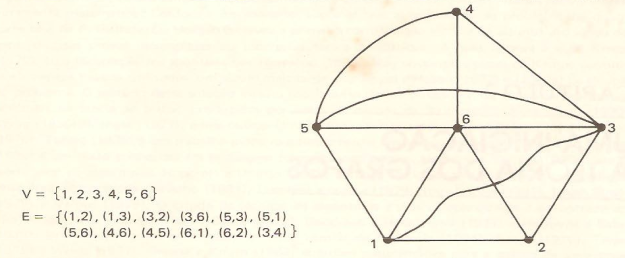
\includegraphics[width=0.7\textwidth]{images/02/fig1.png}
    \end{tabular}
  \end{center}
  \caption{\label{fig:1} Um grafo $G(V,E)$ e sua representação geométrica.}
  \source{Szwarcfiter~\cite{Szwarcfiter1986grafos}.}
\end{figure}


\begin{easylist}
& Vértices: são os elementos de $V$.
& Arestas: são os elementos de $E$.
& Grafo trivial: é um grafo onde $|V| = 1$.
& Vértices adjacentes: dois vértices $v, w$ são ditos adjacentes quando existe uma aresta $e$ tal que $e = (v, w)$; em outras palavras, quando alguma aresta incide em $v$ e $w$.
& Arestas adjacentes: são arestas que possuem uma extremidade em comum, ou seja, que incidem em algum vértice em comum.
& Isomorfismo entre grafos: dois grafos $G_1(V_1, E_1)$ e $G_2(V_2, E_2)$, com $|V_1| = |V_2|$, são ditos isomorfos se e somente se (sse) existe uma função bijetora $f:V_1 \mapsto V_2$ tal que $(v, w) \in E_1$ sse $(f(v), f(w)) \in E_2$ para todo $v, w \in V_1$. Ver Figura~\ref{fig:2}.
\end{easylist}


\begin{figure}[hb]
  \begin{center}
    \begin{tabular}{c}
      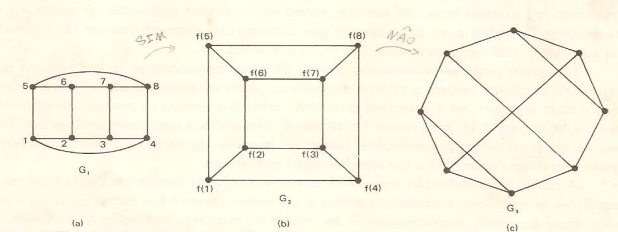
\includegraphics[width=0.8\textwidth]{images/02/fig2.png}
    \end{tabular}
  \end{center}
  \caption{\label{fig:2} Os grafos $G_1$ e $G_2$ são isomorfos um ao outro, mas não a $G_3$.}
  \source{Szwarcfiter~\cite{Szwarcfiter1986grafos}.}
\end{figure}


\begin{easylist}
& Grafo com laços: $G(V,E)$ é um conjunto finito não vazio $V$ e um conjunto $E$ de pares não ordenados de elementos de $V$.
& Grafo dirigido: $G(V,E)$ é um conjunto finito não vazio $V$ e um conjunto $E$ de pares ordenados de elementos de $V$.
& Multigrafo: $G(V,E)$ é um conjunto finito não vazio $V$ e um multiconjunto $E$ de pares não ordenados de elementos de $V$.

& Grau de um vértice $v$ é o número de arestas que incidem em $v$. Laços são contados duas vezes. É denotado por $\operatorname{grau}(v)$.
& Vértice isolado: é um vértice com grau zero.
& Grafo regular de grau $r$: é um grafo em que todos os vértices possuem o mesmo grau $r$.

& Caminho: uma sequência de vértices $v_1, \dots, v_k$ tal que $(v_i, v_{i+1}) \in E, 1\leq i < k$ é denominada caminho de $v_1$ a $v_k$. Seu comprimento é $k-1$.
& Alcance: dizemos que um vértice $v$ alcança um vértice $w$ se existe um caminho de $v$ a $w$.
& Caminho simples: caminho onde todos os vértices de $v_1$ a $v_k$ são diferentes.
& Trajeto: caminho onde todas as arestas são distintas.
& Ciclo: é um caminho $v_1, \dots, v_{k+1}$ em que $v_1 = v_{k+1}$ e $k \geq 3$.
& Ciclo simples: é um ciclo onde todos os vértices são diferentes, exceto o primeiro e o último.
& Grafo acíclico: é um grafo que não possui ciclos simples.
& Ciclos idênticos: ciclos obtidos um do outro por uma rotação de seus vértices.
& Caminho Hamiltoniano: caminho que contém cada vértice do grafo exatamente uma vez.
& Ciclo Hamiltoniano: ciclo $v_1, \dots, v_{k+1}$ onde o caminho $v_1, \dots, v_k$ é Hamiltoniano.
& Caminho ou ciclo Euleriano: caminho ou ciclo que contém cada aresta do grafo exatamente uma vez.
  
  
\begin{figure}[!h]
  \begin{subfigure}{.5\textwidth}
    \centering
    \begin{tabular}{c}
      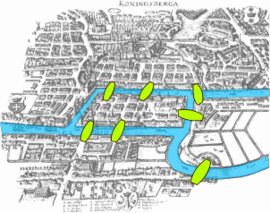
\includegraphics[width=1\textwidth]{images/02/Konigsberg_bridges.png}
    \end{tabular}
    \caption{\label{fig:kon:bridges} Pontes de Konigsberg.}
  \end{subfigure}
  \begin{subfigure}{.5\textwidth}
    \centering
    \begin{tabular}{c}
      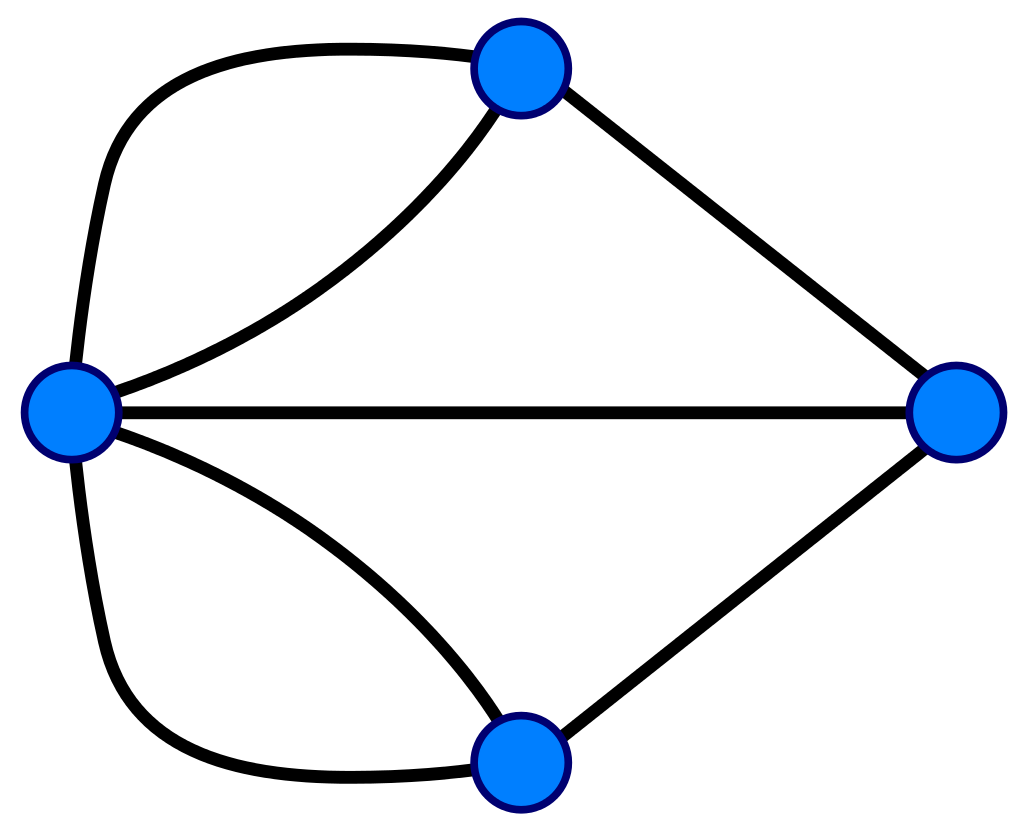
\includegraphics[width=1\textwidth]{images/02/Konigsberg_graph_svg.png}
    \end{tabular}
    \caption{\label{fig:kon:graph} Representação geométrica.}
  \end{subfigure}
  \caption{\label{fig:gray} Existe caminho que percorra todas as pontes uma única vez?}
  \source{Wikipedia.}
\end{figure}


& Grafo conexo: grafo onde, entre cada par de vértices, existe um caminho.
& Grafo desconexo: grafo que não é conexo. Em outras palavras, grafo em que existe algum par de vértices entre os quais não existe caminho.
& Grafo totalmente desconexo: grafo que não possui arestas.
& Subconjunto maximal em relação à propriedade $P$: seja $S$ um conjunto e $S' \subseteq S$, $S'$ é dito maximal em relação à propriedade $P$ quando $S'$ satisfaz $P$ e não existe subconjunto $S'' \supset S$ que satisfaça $P$.
& Componente conexo: subgrafo de um grafo $G$ maximal com relação à conectividade.
& Subconjunto minimal em relação à propriedade $P$: definido de forma análoga ao subconjunto maximal.
& Distância entre dois vértices $v$ e $w$: denotada por $d(v, w)$ é o comprimento do menor caminho entre $v$ e $w$.

% Página 3

& Subtração e adição de vértices e arestas: seja $G(V, E)$ um grafo.
&& Seja $e \in E$ uma aresta, denota-se por $G - e$ o grafo obtido de $G$ pela exclusão da aresta $e$.
&& Seja $(v, w)$ um par de vértices não adjacentes de $G$, denota-se por $G + (v, w)$ o grafo obtido de $G$ adicionando-se a aresta $(v, w)$.
&& Seja $v \in V$ um vértice, denota-se por $G - v$ o grafo obtido da remoção do vértice $v$ e de dotas as arestas nele incidentes.
&& Seja $v \notin V$ um vértice, denota-se por $G + v$ o grafo obtido de $G$ adicionando-se o vértice $v$.

& Teorema 2.1: Un grafo conexo $G$ possui ciclo Euleriano sse todo vértice de $G$ possui grau par.
&& $\Rightarrow$ Seja $C$ um ciclo Euleriano de $G$. Para cada ocorrência de um vértice $v$ em $C$, somamos 2 a seu grau pelo fato de uma ocorrência corresponder a uma aresta de entrada e uma de saída. Portanto, todo vértice de $G$ possui grau par.
&& $\Leftarrow$ Assuma que todos os vértices de $G$ têm grau par. Começamos de um vértice arbitrário $v$ e percorremos um ciclo começando e terminando em $v$, sem repetir arestas. Se todas as arestas foram visitadas, então $G$ é Euleriano. Se não, removemos de $G$ as arestas pertencentes a $C$ e vértices isolados após a remoção, ficando com o grafo $G'$. Todos os vértices de $G'$ têm grau par. Partimos então de algum vértice $u \in G'$ pertencente ao ciclo $C$ e percorremos outro ciclo. O processo é repetido até que o grafo fique vazio. Um ciclo Euleriano pode ser obtido da concatenação de todos os ciclos encontrados. Portanto, $G$ possui ciclo Euleriano.

& Grafo completo: é um grafo que possui uma aresta entre cada par de seus vértices. É denotado por $K_n$, onde $n = |V|$. Possui ${n}\choose{2}$ arestas.
& Complemento de um grafo $G(V, E)$: é o grafo $\bar{G}$ que também possui $V$ como conjunto de vértices e possui como conjunto de arestas $V^2 - E$, onde $V^2$ denota o conjunto de todos os pares não ordenados de elementos distintos de $V$.
& Grafo bipartido: um grafo $G(V, E)$ é bipartido quando seu conjunto de vértices pode ser particionado em dois conjuntos $V_1$ e $V_2$, tais que toda aresta incide em um vértice de $V_1$ e em um vértice de $V_2$.
& Grafo bipartido completo: possui uma aresta para par de vértices $(v_1, v_2)$, onde $v_1 \in V_1$ e $v_2 \in V_2$. É denotado por $K_{n_1, n_2}$, onde $n_1 = |V_1|$ e $n_2 = |V_2|$. Possui $n_1 \times n_2$ arestas.




\end{easylist}






%%%%%%%%%%%%%%%%%%%%%%%%%%%%%%%%%%%%%%%%%%%%%%%%%%%%%%%%%%%%
%Capítulo: Técnicas básicas
%%%%%%%%%%%%%%%%%%%%%%%%%%%%%%%%%%%%%%%%%%%%%%%%%%%%%%%%%%%%

\chapter{Técnicas básicas}

Capítulo 3 de Szwarcfiter, \textit{Grafos e Algoritmos Computacionais}~\cite{Szwarcfiter1986grafos}.

%%%%%%%%%%%%%%%%%%%%%%%%%%%%%%%%%%%%%%%%%%%%%%%%%%%%%%%%%%%%
\section{Introdução}

Serão vistos neste capítulo alguns algoritmos básicos em grafos.

%%%%%%%%%%%%%%%%%%%%%%%%%%%%%%%%%%%%%%%%%%%%%%%%%%%%%%%%%%%%
\section{Ordenação topológica}

% Página 8

\begin{easylist}

  & Como visto na seção~\ref{sec:digraph}, sabemos que um digrafo acíclico $D(V, E)$ induz um conjunto parcialmente ordenado $(V, <)$. A relação $<$ é definida por $v < w \Leftrightarrow v$ alcança $w$ em $D$ para todo $v, w \in V$. Com isso, é possível ordenar os vértices do digrafo de modo a obter uma sequência $v1, \dots, v_n$, onde $n = |V|$ satisfazendo

  \[ v_i, < v_j \Rightarrow i<j \text{ para } i, j \in [1, n] \]

\begin{algorithm}[H]
\SetAlgoLined
\KwData{digrafo acíclico $D(V, E)$ }
 \For{ $j = 1, \dots, |V|$ }{
  escolher vértice $w$ com grau de entrada nulo\;
  remover $w$ de $V$\;
  $v_j \gets w$\;
 }
 \caption{Ordenação topológica em digrafo}
\end{algorithm}
  
\end{easylist}

%%%%%%%%%%%%%%%%%%%%%%%%%%%%%%%%%%%%%%%%%%%%%%%%%%%%%%%%%%%%
\section{Busca em árvores}

\clearpage

\begin{easylist}

  & Busca em árvores:
  
  && Busca em profundidade: visitamos primeiro a raiz. Do vértice atual, caso tenha filhos, visitamos seu primeiro filho não visitado; caso não tenha, retornamos para seu pai.

  && Busca em largura: visitamos primeiro a raiz. Colocamos os filhos do vértice atual em uma fila. Visitamos cada vértice da fila até que se esvazie.


  {\EXERCICIOS}
  
  \begin{enumerate}
  \item Considere a árvore abaixo. Em que ordem os vértices serão visitados pela primeira vez
    \begin{enumerate}
      \item em uma busca em profundidade?
      \item em uma busca em largura?
    \end{enumerate}
  \end{enumerate}

\begin{verbatim}

                                       a
                                      / \ 
                                     /   \
                                    /     \
                                   /       \
                                  /         \
                                 b           c
                                / \         /|\
                               /   \       / | \   
                              d     e     f  g  h
                             / \    |    /     / \
                            i   j   k   l     m   n

\end{verbatim}


  & Busca em grafos: em um grafo não há raiz, pai, filhos, direita, esquerda ou níveis, como em uma árvore. Para se ter controle dos vértices já visitados, evitando visitas múltiplas a um mesmo vértice, é necessário associar a cada vértice atributos ou marcas.

  && Busca em largura:

\begin{algorithm}[H]
\SetAlgoLined
\KwData{grafo conexo $G(V, E)$ }
  escolher, enfileirar e marcar vértice inicial arbitrário;

  \While{\textnormal{fila não vazia}}
  {
    $v \gets$ desenfileira();
    
    marcar e enfileirar vizinhos de $v$ não marcados;
  }
  \caption{Busca em largura em grafo}
\end{algorithm}

\clearpage

&& Busca em profundidade: visitamos primeiro a raiz. Do vértice atual, caso tenha filhos, visitamos seu primeiro filho não visitado; caso não tenha, retornamos para seu pai.

\end{easylist}


\begin{algorithm}[H]
\SetAlgoLined
\KwData{grafo conexo $G(V, E)$ }
  escolher vértice inicial arbitrário $v$;

  executar $P(v)$;

  \SetKwProg{Def}{def}{:}{end}
  \Def{$P(x)$}
  {
    marcar $x$\;
    empilhar $x$\;
    \For{$w \in \operatorname{adjacencia}(x)$}{
      \If{$w$ \textnormal{não é marcado}}
      { 
        $P(w)$;
      }
    }
    desempilhar $x$\;
  }
  \caption{Busca em profundidade em grafo}
\end{algorithm}

%%%%%%%%%%%%%%%%%%%%%%%%%%%%%%%%%%%%%%%%%%%%%%%%%%%%%%%%%%%%
\section{Busca irrestrita}

\begin{easylist}

  & Busca irrestrita: o algoritmo de busca irrestrita que veremos aqui é uma variação da busca em profundidade que permite que um mesmo vértice seja visitado várias vezes. Uma busca irrestrita em profundidade constrói uma árvore denominada árvore irrestrita de profundidade. A Figura~\ref{fig:3:1} mostra um exemplo desse tipo de árvore.

\end{easylist}


\begin{algorithm}[H]
\SetAlgoLined
\KwData{grafo conexo $G(V, E)$ }
  escolher vértice inicial arbitrário $v$;

  executar $P(v)$;

  \SetKwProg{Def}{def}{:}{end}
  \Def{$P(x)$}
  {
    marcar $x$\;
    empilhar $x$\;
    \For{$w \in \operatorname{adjacencia}(x)$}{
      \If{$w$ \textnormal{não é marcado}}
      { 
        $P(w)$;
      }
    }
    desempilhar $x$\;
    desmarcar $x$\;
  }
  \caption{Busca irrestrita em grafo}
\end{algorithm}


\begin{figure}[b]
  \begin{center}
    \begin{tabular}{c}
      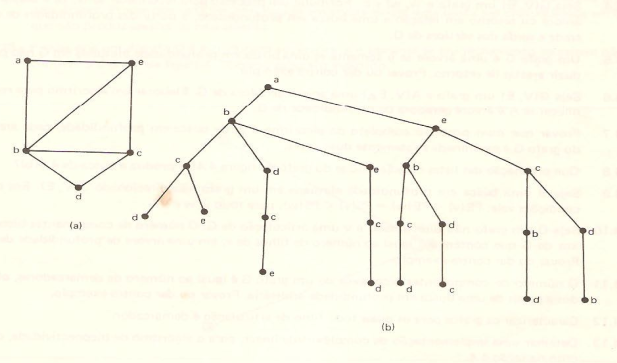
\includegraphics[width=0.7\textwidth]{images/03/unrestricted.png}
    \end{tabular}
  \end{center}
  \caption{\label{fig:3:1} (a) Um grafo $G(V,E)$; (b) árvore irrestrita de profundidade.}
  \source{Szwarcfiter~\cite{Szwarcfiter1986grafos}.}
\end{figure}
  





%%%%%%%%%%%%%%%%%%%%%%%%%%%%%%%%%%%%%%%%%%%%%%%%%%%%%%%%%%%%
%\section{Busca em árvores}


%%%%%%%%%%%%%%%%%%%%%%%%%%%%%%%%%%%%%%%%%%%%%%%%%%%%%%%%%%%%
%\section{Busca em grafos}


%%%%%%%%%%%%%%%%%%%%%%%%%%%%%%%%%%%%%%%%%%%%%%%%%%%%%%%%%%%%
%\section{Exercícios}

%\begin{enumerate}
%  \item 
%    \begin{enumerate}
%      \item 
%      \item 
%    \end{enumerate}
%  \item 
%  \item 
%\end{enumerate}




%%%%%%%%%%%%%%%%%%%%%%%%%%%%%%%%%%%%%%%%%%%%%%%%%%%%%%%%%%%%
%Capítulo: Buscas em grafos
%%%%%%%%%%%%%%%%%%%%%%%%%%%%%%%%%%%%%%%%%%%%%%%%%%%%%%%%%%%%

%\input{04_buscas.tex}


%%%%%%%%%%%%%%%%%%%%%%%%%%%%%%%%%%%%%%%%%%%%%%%%%%%%%%%%%%%%
%Capítulo: Outras técnicas
%%%%%%%%%%%%%%%%%%%%%%%%%%%%%%%%%%%%%%%%%%%%%%%%%%%%%%%%%%%%

\chapter{Outras técnicas}

Capítulo 5 de Szwarcfiter, \textit{Grafos e Algoritmos Computacionais}~\cite{Szwarcfiter1986grafos}.

%%%%%%%%%%%%%%%%%%%%%%%%%%%%%%%%%%%%%%%%%%%%%%%%%%%%%%%%%%%%
\section{Introdução}

Serão vistos neste capítulo alguns algoritmos em grafos.

%%%%%%%%%%%%%%%%%%%%%%%%%%%%%%%%%%%%%%%%%%%%%%%%%%%%%%%%%%%%
\section{Árvore geradora mínima}

\begin{easylist}

  & Grafo ponderado: é um grafo que possui uma função relacionando o conjunto de vértices ou de arestas a algum valor numérico, conhecido como peso ou custo.

  & Árvore geradora mínima (AGM): seja $G(V, E)$ um grafo conexo em que cada aresta possui um peso, o problema da árvore geradora mínima consiste em encontrar uma árvore que conecte todos os vértices de $V$ cuja soma dos pesos é a menor possível.

  && Algoritmo de Kruskal: usa \textit{union-find trees} com \textit{path compression} e \textit{union by rank}.

%%%%%%%%%%%%%%%%%%%%
\begin{algorithm}[H]
\SetAlgoLined
\KwData{grafo conexo $G(V, E)$ com função de custo associada às arestas}

  ordenar as arestas por ordem não decrescente de custo;

  associar cada vértice a um conjunto distinto;

  \For{$e \in E$ \textnormal{em ordem não decrescente de peso}}
  {
    \If{$e$ \textnormal{liga vértices de conjuntos diferentes}}
    {
      unir os dois conjuntos;
      
      marcar $e$ como parte da AGM;
    }
  }
  \caption{Algoritmo de Kruskal}
\end{algorithm}
%%%%%%%%%%%%%%%%%%%%

  && Algoritmo de Prim: usa uma fila de prioridades implementada com \textit{heap}.

%%%%%%%%%%%%%%%%%%%%
\begin{algorithm}[H]
\SetAlgoLined
\KwData{grafo conexo $G(V, E)$ com função de custo associada às arestas}

  inicializar $V_2 = \{x\}$ onde $x$ é um vértice arbitrário;

  inicializar $E_2 = \{\}$;

  \While{$V_2 \neq V$}
  {
    escolher aresta $(u, v)$ tal que $u \in V_2$ e $v \notin V_2$ cujo peso seja mínimo;

    adicionar $v$ a $V_2$ e $(u, v)$ a $E_2$;
  }

  Retornar $G_2(V_2, E_2)$, que representa a AGM;
  \caption{Algoritmo de Prim}
\end{algorithm}
%%%%%%%%%%%%%%%%%%%%



%%%%%%%%%%%%%%%%%%%%%%%%%%%%%%%%%%%%%%%%%%%%%%%%%%%%%%%%%%%%
\section{Menor distância em grafos}


%%%%%%%%%%%%%%%%%%%%
\begin{algorithm}[H]
\SetAlgoLined
\KwData{grafo $G(V, E)$, origem $s$}
  \SetKwProg{Def}{def}{:}{end}
  \Def{$Inicializa(G, s)$}
  {
    \For{$w \in V$}
    {
      dist($v$) = $\infty$;

      pai($v$) = NULL;
    }
    dist($s$) = 0;
  }

  \Def{$Relax(u, v)$}
  {
    \If{\textnormal{dist($v$) $>$ dist($u$) + peso(($u$, $v$))}}
    { 
      dist($v$) = dist($u$) + peso(($u$, $v$));

      pai($v$) = $u$;
    }
  }
  
  \Def{$Dijkstra(G, s)$}
  {
    \textit{Inicializa(G, s)}

    $Q = V$            /* Inserir todos os vértices em fila de prioridade. */
    
    \hspace{1cm}       /* Prioridade maior quanto menor o peso. */

    \While{fila $Q$ não vazia}
    {
      u = desenfileira(Q) /* Vértice mais próximo a $s$ */

      \For{$v \in \operatorname{adjacencia}(u)$}
      {
        \textit{Relax(u, v)}
      }
    }
  }
  \caption{Algoritmo de Dijkstra}
\end{algorithm}
%%%%%%%%%%%%%%%%%%%%



\end{easylist}



%%%%%%%%%%%%%%%%%%%%%%%%%%%%%%%%%%%%%%%%%%%%%%%%%%%%%%%%%%%%
%\section{Busca em árvores}


%%%%%%%%%%%%%%%%%%%%%%%%%%%%%%%%%%%%%%%%%%%%%%%%%%%%%%%%%%%%
%\section{Busca em grafos}


%%%%%%%%%%%%%%%%%%%%%%%%%%%%%%%%%%%%%%%%%%%%%%%%%%%%%%%%%%%%
%\section{Exercícios}

%\begin{enumerate}
%  \item 
%    \begin{enumerate}
%      \item 
%      \item 
%    \end{enumerate}
%  \item 
%  \item 
%\end{enumerate}




%%%%%%%%%%%%%%%%%%%%%%%%%%%%%%%%%%%%%%%%%%%%%%%%%%%%%%%%%%%%
%Capítulo: Fluxo máximo em redes
%%%%%%%%%%%%%%%%%%%%%%%%%%%%%%%%%%%%%%%%%%%%%%%%%%%%%%%%%%%%

\chapter{Fluxo em redes}

Capítulo 6 de Szwarcfiter, \textit{Grafos e Algoritmos Computacionais}~\cite{Szwarcfiter1986grafos}.

%%%%%%%%%%%%%%%%%%%%%%%%%%%%%%%%%%%%%%%%%%%%%%%%%%%%%%%%%%%%
\section{Introdução}

Serão vistos neste capítulo definições e algoritmos relacionados a fluxo em redes.

%%%%%%%%%%%%%%%%%%%%%%%%%%%%%%%%%%%%%%%%%%%%%%%%%%%%%%%%%%%%
\section{O problema do fluxo máximo}

% Página 22

\begin{easylist}

  & Multidigrafo $D(V,E)$ é um conjunto finito não vazio $V$ e um multiconjunto $E$ de pares ordenados de elementos distintos de $V$. Portanto, pode haver mais de uma aresta $(v, w)$ simultaneamente.

  & Rede é um multidigrafo $D(V, E)$ em que a cada aresta $e$ está associado uma capacidade $c(e)$.

  & Fluxo: considere uma rede $D(V, E)$ contendo dois vértices especiais $s, t \in V$ denominados origem e destino respectivamente. Os vértices $s$ e $t$ possuem as seguintes propriedades:

  && $s$ é uma fonte que alcança todos os vértices;
  && $t$ é um sumidouro alcançado por todos os vértices.

  Um fluxo $f$ de $s$ a $t$ em $D$ é uma função que, a cada aresta $e \in E$ associa um número real não negativo $f(e)$ com as seguintes propriedades:
  
  && $0 \leq f(e) \leq c(e)$
  && $\sum_{w_1} f(w_1, v) = \sum_{w_2} f(v, w_2)$ para todo $v \neq s, t$. 

  & Fluxo ilegal: fluxo que não satisfaz as propriedades da definição.

  & Valor do fluxo no vértice $v$ é dado pela somatória dos fluxos nas arestas convergentes a $v$ ou divergentes de $v$. De forma análoga, é dada pela soma dos fluxos das arestas divergentes de $s$ ou convergentes a $t$.

  & Valor do fluxo no digrafo $D(V, E)$ é denotado por $f(D)$ e é igual a $f(s)$.

  & Aresta saturada: é uma aresta em que $f(e) = c(e)$.

  & Vértice saturado: é um vértice com todas as arestas convergentes e/ou divergentes saturadas.

  & Fluxo maximal: fluxo onde todo caminho de $s$ a $t$ possui alguma aresta saturada.

  & Corte: seja $S \subseteq V$ um subconjunto de vértices tal que $s \in S$, $t \notin S$ e $\bar S = V - S$ seu complemento, um corte $(S, \bar S)$ em $D$ é o subconjunto das arestas que possuem uma extremidade em $S$ e outra em $\bar S$.

  & Capacidade de um corte $c(S, \bar S)$: sejam
  $(S, \bar S)^+ = \{(v, w) \in E | v \in S, w \in \bar S\}$ e
  $(S, \bar S)^- = \{(v, w) \in E | v \in \bar S, w \in S\}$, a capacidade $c(S, \bar S)$ é o somatório das capacidades das arestas de $(S, \bar S)^+$, ou seja,
  \[ c(S, \bar S) = \sum_{e \in (S, \bar S)^+} c(e) \].

  & Fluxo no corte $f(S, \bar S)$: seja $f$ um fluxo e $(S, \bar S)$ um corte, o fluxo $f(S, \bar S)$ no corte $(S, \bar S)$ é definido como a diferença 
  \[ f(S, \bar S) = \sum_{e \in (S, \bar S)^+} f(e) - \sum_{e \in (S, \bar S)^-} f(e) \].

  & Lema: seja $f$ um fluxo e $(S, \bar S)$ um corte em um digrafo $D$. Temos que $f(S, \bar S) = f(D)$.

  & Aresta direta: aresta $e$ tal que $c(e) - f(e) > 0$

  & Aresta contrária: aresta $e$ tal que $f(e) > 0$

  & Digrafo residual $D'(F)$: seja $D(V, E)$ um digrafo e $f$ um fluxo,
  && se $(v, w)$ é aresta direta de $D$ então $(v, w)$ é aresta direta de $D'$ com capacidade $c'(v, w) = c(v, w) - f(v, w)$.
  && se $(v, w)$ é aresta contrária de $D$ então $(w, v)$ é aresta contrária de $D'$ com capacidade $c'(w, v) = f(v, w)$.

\begin{figure}[t]
  \begin{center}
    \begin{tabular}{c}
      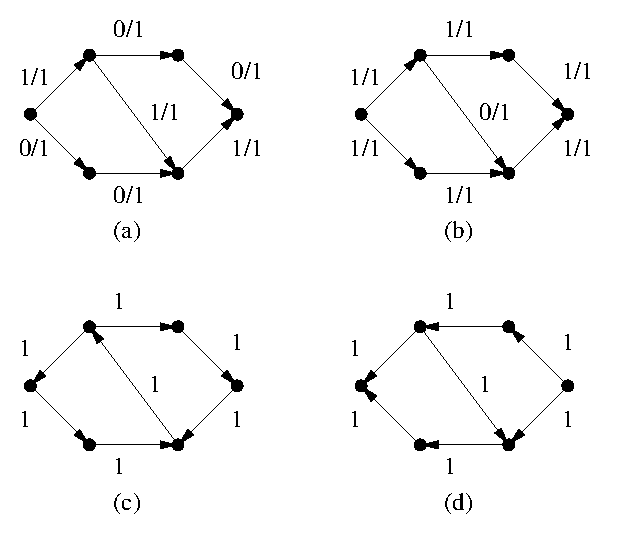
\includegraphics[width=0.7\textwidth]{images/06/flow01.eps}
    \end{tabular}
  \end{center}
  \caption{\label{fig:3:1} (a) Fluxo maximal; (b) fluxo máximo; (c) digrafo residual no fluxo maximal; (d) digrafo residual no fluxo máximo.}
  \source{Szwarcfiter~\cite{Szwarcfiter1986grafos}.}
\end{figure}

  & Caminho aumentante para $f$ é um caminho no digrafo residual $D'$ que permite aumentar o fluxo no digrafo $D$.

  & Lema: seja $f$ um fluxo em um digrafo $D$ e $D'$ seu digrafo residual correspondente. Se existe caminho aumentante de $s$ a $t$, o fluxo pode ser aumentado de um valor igual à menor capacidade das arestas do caminho.

  & Corte mínimo: corte com a menor capacidade no digrafo $D$.

  & Fluxo máximo: fluxo com o maior valor possível no digrafo $D$. O fluxo máximo não pode ultrapassar a capacidade do corte mínimo.
  \[ f(D) = f(S, \bar S) = \sum_{e \in (S, \bar S)^+} f(e) - \sum_{e \in (S, \bar S)^-} f(e) \leq \sum_{e \in (S, \bar S)^+} c(e) = c(S, \bar S) \]

  & Teorema: o valor do fluxo máximo em um digrafo $D$ é igual à capacidade do corte mínimo de $D$.

  & Corolário: um fluxo $f$ em um digrafo $D$ é máximo sse não existir caminho aumentante para $f$ no digrafo residual $D'$.

\begin{algorithm}[H]
\SetAlgoLined
\KwData{digrafo $D(V, E)$ com capacidades c(e) positivas para todo $e\in E$; origem $s\in V$; destino $t\in V$}
  F = 0
  \For{$e \in E$}
  {
    f(e) = 0
  }
  construir o digrafo residual $D'(f)$;

  \While{\textnormal{existe caminho $(v_1, \dots, v_k)$ de $s=v_1$ a $t=v_k$ em $D'$}}
  {
    $F' = min\{c'(v_j, v_{j+1}) | 1 \leq j < k\}$;

    \For{$j \in {1, \dots, k-1}$}
    {
      \eIf{$(v_j, v_{j+1})$ \textnormal{é aresta direta}}
      { 
        $f(v_j, v_{j+1}) += F'$;
      }{ 
        $f(v_{j+1}, v_j) -= F'$;
      }
    }
    F = F + F';
    
    recalcular $D'$;
  }
  \caption{Fluxo máximo em rede}
\end{algorithm}
  
\end{easylist}





\iffalse

  
\clearpage  
  
$\bar{A}$ vs $\overline{A}$

$\bar{\mathcal A}$ vs $\overline{\mathcal A}$

$\bar{ABC}$ vs $\overline{ABC}$
  

  

  
  

  & Como visto na seção~\ref{sec:digraph}, sabemos que um digrafo acíclico $D(V, E)$ induz um conjunto parcialmente ordenado $(V, <)$. A relação $<$ é definida por $v < w \Leftrightarrow v$ alcança $w$ em $D$ para todo $v, w \in V$. Com isso, é possível ordenar os vértices do digrafo de modo a obter uma sequência $v1, \dots, v_n$, onde $n = |V|$ satisfazendo

  \[ v_i, < v_j \Rightarrow i<j \text{ para } i, j \in [1, n] \]

\begin{algorithm}[H]
\SetAlgoLined
\KwData{digrafo acíclico $D(V, E)$ }
 \For{ $j = 1, \dots, |V|$ }{
  escolher vértice $w$ com grau de entrada nulo\;
  remover $w$ de $V$\;
  $v_j \gets w$\;
 }
 \caption{Ordenação topológica em digrafo}
\end{algorithm}
  
\end{easylist}

%%%%%%%%%%%%%%%%%%%%%%%%%%%%%%%%%%%%%%%%%%%%%%%%%%%%%%%%%%%%
\section{Busca em árvores}

\clearpage

\begin{easylist}

  & Busca em árvores:
  
  && Busca em profundidade: visitamos primeiro a raiz. Do vértice atual, caso tenha filhos, visitamos seu primeiro filho não visitado; caso não tenha, retornamos para seu pai.

  && Busca em largura: visitamos primeiro a raiz. Colocamos os filhos do vértice atual em uma fila. Visitamos cada vértice da fila até que se esvazie.


  {\EXERCICIOS}
  
  \begin{enumerate}
  \item Considere a árvore abaixo. Em que ordem os vértices serão visitados pela primeira vez
    \begin{enumerate}
      \item em uma busca em profundidade?
      \item em uma busca em largura?
    \end{enumerate}
  \end{enumerate}

\begin{verbatim}

                                       a
                                      / \ 
                                     /   \
                                    /     \
                                   /       \
                                  /         \
                                 b           c
                                / \         /|\
                               /   \       / | \   
                              d     e     f  g  h
                             / \    |    /     / \
                            i   j   k   l     m   n

\end{verbatim}


  & Busca em grafos: em um grafo não há raiz, pai, filhos, direita, esquerda ou níveis, como em uma árvore. Para se ter controle dos vértices já visitados, evitando visitas múltiplas a um mesmo vértice, é necessário associar a cada vértice atributos ou marcas.

  && Busca em largura:

\begin{algorithm}[H]
\SetAlgoLined
\KwData{grafo conexo $G(V, E)$ }
  escolher, enfileirar e marcar vértice inicial arbitrário;

  \While{\textnormal{fila não vazia}}
  {
    $v \gets$ desenfileira();
    
    marcar e enfileirar vizinhos de $v$ não marcados;
  }
  \caption{Busca em largura em grafo}
\end{algorithm}

\clearpage

&& Busca em profundidade:

\end{easylist}


\begin{algorithm}[H]
\SetAlgoLined
\KwData{grafo conexo $G(V, E)$ }
  escolher vértice inicial arbitrário $v$;

  executar $P(v)$;

  \SetKwProg{Def}{def}{:}{end}
  \Def{$P(x)$}
  {
    marcar $x$\;
    empilhar $x$\;
    \For{$w \in \operatorname{adjacencia}(x)$}{
      \If{$w$ \textnormal{não é marcado}}
      { 
        $P(w)$;
      }
    }
    desempilhar $x$\;
  }
  \caption{Busca em profundidade em grafo}
\end{algorithm}

%%%%%%%%%%%%%%%%%%%%%%%%%%%%%%%%%%%%%%%%%%%%%%%%%%%%%%%%%%%%
\section{Busca irrestrita}

\begin{easylist}

  & Busca irrestrita: o algoritmo de busca irrestrita que veremos aqui é uma variação da busca em profundidade que permite que um mesmo vértice seja visitado várias vezes. Uma busca irrestrita em profundidade constrói uma árvore denominada árvore irrestrita de profundidade. A Figura~\ref{fig:3:1} mostra um exemplo desse tipo de árvore.

\end{easylist}


\begin{algorithm}[H]
\SetAlgoLined
\KwData{grafo conexo $G(V, E)$ }
  escolher vértice inicial arbitrário $v$;

  executar $P(v)$;

  \SetKwProg{Def}{def}{:}{end}
  \Def{$P(x)$}
  {
    marcar $x$\;
    empilhar $x$\;
    \For{$w \in \operatorname{adjacencia}(x)$}{
      \If{$w$ \textnormal{não é marcado}}
      { 
        $P(w)$;
      }
    }
    desempilhar $x$\;
    desmarcar $x$\;
  }
  \caption{Busca irrestrita em grafo}
\end{algorithm}


\begin{figure}[b]
  \begin{center}
    \begin{tabular}{c}
      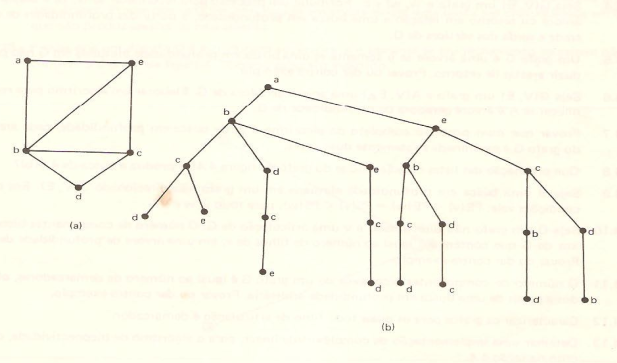
\includegraphics[width=0.7\textwidth]{images/03/unrestricted.png}
    \end{tabular}
  \end{center}
  \caption{\label{fig:3:1} (a) Um grafo $G(V,E)$; (b) árvore irrestrita de profundidade.}
  \source{Szwarcfiter~\cite{Szwarcfiter1986grafos}.}
\end{figure}
  
\fi




%%%%%%%%%%%%%%%%%%%%%%%%%%%%%%%%%%%%%%%%%%%%%%%%%%%%%%%%%%%%
%\section{Busca em árvores}


%%%%%%%%%%%%%%%%%%%%%%%%%%%%%%%%%%%%%%%%%%%%%%%%%%%%%%%%%%%%
%\section{Busca em grafos}


%%%%%%%%%%%%%%%%%%%%%%%%%%%%%%%%%%%%%%%%%%%%%%%%%%%%%%%%%%%%
%\section{Exercícios}

%\begin{enumerate}
%  \item 
%    \begin{enumerate}
%      \item 
%      \item 
%    \end{enumerate}
%  \item 
%  \item 
%\end{enumerate}




%%%%%%%%%%%%%%%%%%%%%%%%%%%%%%%%%%%%%%%%%%%%%%%%%%%%%%%%%%%%
%Capítulo: Problemas NP-completo
%%%%%%%%%%%%%%%%%%%%%%%%%%%%%%%%%%%%%%%%%%%%%%%%%%%%%%%%%%%%

%\input{07_problemas.tex}


%%%%%%%%%%%%%%%%%%%%%%%%%%%%%%%%%%%%%%%%%%%%%%%%%%%%%%%%%%%%
%Capítulo: Entrada e saída
%%%%%%%%%%%%%%%%%%%%%%%%%%%%%%%%%%%%%%%%%%%%%%%%%%%%%%%%%%%%

%\input{io.tex}


%%%%%%%%%%%%%%%%%%%%%%%%%%%%%%%%%%%%%%%%%%%%%%%%%%%%%%%%%%%%
%Capítulo: Vetores
%%%%%%%%%%%%%%%%%%%%%%%%%%%%%%%%%%%%%%%%%%%%%%%%%%%%%%%%%%%%

%\input{array.tex}


%%%%%%%%%%%%%%%%%%%%%%%%%%%%%%%%%%%%%%%%%%%%%%%%%%%%%%%%%%%%
%Capítulo: Funções
%%%%%%%%%%%%%%%%%%%%%%%%%%%%%%%%%%%%%%%%%%%%%%%%%%%%%%%%%%%%

%\input{function.tex}


%%%%%%%%%%%%%%%%%%%%%%%%%%%%%%%%%%%%%%%%%%%%%%%%%%%%%%%%%%%%
%Capítulo: Exercícios
%%%%%%%%%%%%%%%%%%%%%%%%%%%%%%%%%%%%%%%%%%%%%%%%%%%%%%%%%%%%

%\input{exercise.tex}




%%%%%%%%%%%%%%%%%%%%%%%%%%%%%%%%%%%%%%%%%%%%%%%%%%%%%%%%%%%%
%Capítulo: Exemplos de programas
%%%%%%%%%%%%%%%%%%%%%%%%%%%%%%%%%%%%%%%%%%%%%%%%%%%%%%%%%%%%

%\chapter{Exemplos de programas}


%%%%%%%%%%%%%%%%%%%%%%%%%%%%%%%%%%%%%%%%%%%%%%%%%%%%%%%%%%%%
%Seção: pause.cpp

%\section{pause.cpp}

%\lstinputlisting[caption=series.cpp]{src/pause.cpp}

%%%%%%%%%%%%%%%%%%%%%%%%%%%%%%%%%%%%%%%%%%%%%%%%%%%%%%%%%%%%
%Seção: ascii.cpp

%\section{ascii.cpp}

%\lstinputlisting[caption=ascii.cpp]{src/ascii.cpp}

%%%%%%%%%%%%%%%%%%%%%%%%%%%%%%%%%%%%%%%%%%%%%%%%%%%%%%%%%%%%
%Seção: dado.cpp

%\section{dado.cpp}

%\lstinputlisting[caption=dado.cpp]{src/dado.cpp}

%%%%%%%%%%%%%%%%%%%%%%%%%%%%%%%%%%%%%%%%%%%%%%%%%%%%%%%%%%%%
%Seção: primos.cpp

%\section{primos.cpp}

%\lstinputlisting[caption=series.cpp]{src/primos.cpp}

%%%%%%%%%%%%%%%%%%%%%%%%%%%%%%%%%%%%%%%%%%%%%%%%%%%%%%%%%%%%
%Seção: series.cpp

%\section{series.cpp}

%\lstinputlisting[caption=series.cpp]{src/series.cpp}




%%%%%%%%%%%%%%%%%%%%%%%%%%%%%%%%%%%%%%%%%%%%%%%%%%%%%%%%%%%%
%Seção: generate.cpp

%\section{generate.cpp}

%\lstinputlisting[caption=generate.cpp]{src/generate.cpp}

%%%%%%%%%%%%%%%%%%%%%%%%%%%%%%%%%%%%%%%%%%%%%%%%%%%%%%%%%%%%
%Seção: ordena.cpp

%\section{ordena.cpp}

%\lstinputlisting[caption=ordena.cpp]{src/ordena.cpp}

%\nocite{gonzalez2006image,
%dougherty2003handson,
%learning_opencv,
%Duda:2001,
%Costa:2001,
%Jain1995machine,
%soille1999morphological,
%Tufte:83,
%GeometryMultiple,
%MultipleView,
%3dComputer}

\bibliography{refs}
\bibliographystyle{plain}


\end{document}

